\documentclass{jot}
% Use the documentclass option 'lineno' to view line numbers

% Enter the JOT metadata in the following 
\usepackage{multirow}

\jotdetails{
    volume=vv,      % volume
    number=nn,       % number or issue
    articleno=aa,   % article number, eg a1 for research articles, e for editorials
    year=2022,      % year
    license=ccby    % choose from ccby, ccbynd, ccbyncnd
}
\newcommand{\command}[1]{{\color{codepurple}\texttt{\textbackslash #1}}}
\newcommand{\param}[1]{{\color{blue}\texttt{#1}}}
% Select the article type
\articletype{regular} 
    % {editorial} editorial 
    % {regular} regular contribution
    % {manual} manual
    % {column} column

\title{Towards behavioral consistency in multi-modeling}

\author[$\ast$]{Tim Kräuter}
% Arbitrary co-author order. Everyone contributed significantly.
\author[$\ast\dagger$]{Harald König}
\author[$\ast$]{Adrian Rutle}
\author[$\ast$]{Yngve Lamo}
\author[$\ddagger$]{Patrick Stünkel}

\affil[$\ast$]{Western Norway University of Applied Sciences, Bergen, Norway}
\affil[$\dagger$]{University of Applied Sciences, FHDW, Hannover, Germany}
\affil[$\ddagger$]{Haukeland Universitetssykehus, Bergen, Norway}

\keywords{	
Global behavioral consistency,
Consistency verification,
Multi-modeling,
Heterogeneous models,
Rewriting Logic,
Graph transformation
}

\runningtitle{Towards behavioral consistency in multi-modeling} % For use in the internal pages 

\runningauthor{Kräuter \textit{et al.}}

\usepackage{amsthm} % for proofs
\usepackage{amsmath} % theorems, definitions, etc.
\newtheorem{definition}{Definition}
\newcommand{\definitionautorefname}{Definition}

% Table

\usepackage{glossaries}
\usepackage[nameinlink]{cleveref} % Reference footnotes.
\crefname{figure}{{figure}}{figures}
\Crefname{figure}{{Figure}}{Figures}
\crefformat{footnote}{#2\footnotemark[#1]#3}

\newacronym{ltl}{LTL}{Linear temporal logic}
\newacronym{mde}{MDE}{Model-driven engineering}
\newacronym{bpmn}{BPMN}{Business Process Modeling Notation}
\newacronym{uml}{UML}{Unified Modeling Language}
\newacronym{csp}{CSP}{Communication Sequential Processes}
\newacronym{ccsl}{CCSL}{Clock Constraint Specification Language}
\newacronym{dsl}{DSL}{Domain-specific language}
\newacronym{srm}{SRM}{system relationship model}

% correct bad hyphenation here
\hyphenation{be-ha-vi-o-ral}

% Listing settings

\lstdefinelanguage{Interaction}[]{Java}{
    morekeywords={synchronize},
    comment=[l]{---},
}

\lstset{emph={  
    rl
    },emphstyle={\color{blue}\bfseries}
}

\begin{abstract}
%ABOUT: Introduce multi-model and motivate global behavior checking
Multiple interacting systems are needed to realize the requirements of complex domains.
Describing the interactions between these systems and checking their global behavioral consistency is a general, well-known challenge in software engineering.
To address this challenge, model-driven software engineering utilizes abstract representations of the constituting systems and their interactions, resulting in a \emph{multi-model} representing the overall software.
In such a multi-modeling setting, global consistency rules must be satisfied by a set of heterogeneously typed models to guarantee a desired \emph{global behavior}.
In this paper, we propose a novel approach for behavioral consistency management of heterogeneous multi-models.
The approach introduces a workflow in which we
(i) specify \emph{global behavioral properties},
(ii) align the individual models by specifying their \emph{interactions}, and finally,
(iii) check the \emph{global behavioral properties} which should be satisfied by the multi-model by generating a formal specification of the \emph{global behavior}.
Our approach is independent of the particular formalism used in the generated specification, and we currently support generating graph transformations (Groove) and rewriting logic (Maude).
\end{abstract}

% TODO: Comment in after acceptance and helpful feedback.
% \acknowledgment{We want to thank the anonymous reviewers for their valuable comments and helpful suggestions.}

\begin{document}    
\maketitle
\urlstyle{rm}


\section{Introduction} \label{sec:introduction}
% Introduce multi-model
\gls*{mde} addresses the increasing complexity of software systems by employing models to describe the different aspects of the system.
In this way, \gls*{mde} promotes a clear separation of concerns and raises the abstraction level throughout the entire development process \cite{franceModeldrivenDevelopmentComplex2007}.
These models are then used to generate portions of the system leading to an increase in productivity and reduction of errors \cite{brambillaModeldrivenSoftwareEngineering2017}.
As multiple interacting systems are needed to realize the requirements of complex domains, a set of corresponding models would be needed to represent these systems and their interactions.
Such a collection of inter-related models is referred to as a \emph{multi-model} \cite{boronatWhatMultimodelingLanguage2009, stunkelComprehensiveSystemsFormal2021}, which is usually heterogeneous, meaning it consists of models conforming to different modeling languages.
% Consistency in multi-modeling
Models in a multi-model contradicting each other can lead to problems during development, system generation, and system execution.
Consequently, continuous multi-model consistency management during the development process is a significant issue for multi-models \cite{spanoudakisInconsistencyManagementSoftware2001, cicchettiMultiviewApproachesSoftware2019}.

% Consistency can be checked for a set of structural models
Recent research describes methods to check the structural consistency of a multi-model \cite{stunkelComprehensiveSystemsFormal2021, klareCommonalitiesPreservingConsistency2019}.
Structural models, like UML class diagrams, describe structural aspects of systems, i.e., domain concepts and relations between these concepts.
This is usually referred to as the static semantics of the software system as it only describes the set of valid instances or states of the system.
% Challenge: Consistency for a set of behavioral models.
Nevertheless, approaches to multi-model consistency management must also include a means to maintain \emph{behavioral consistency} since behavioral models, like \gls*{bpmn} models, are associated with execution semantics describing dynamic aspects of the system \cite{objectmanagementgroupUnifiedModelingLanguage2017, objectmanagementgroupBusinessProcessModel2013}.
For example, embedded and cyber-physical systems are composed of heterogeneous interacting components \cite{varalarsenBehavioralCoordinationOperator2015}.

% Existing solutions. But they are not sufficient!
Several approaches exist for checking the consistency of pairs of behavioral models.
For example, consistency checking for sequence diagrams and statecharts was implemented using Petri nets \cite{yaoConsistencyCheckingUML2006} and \gls*{csp} \cite{kusterExplicitBehavioralConsistency2003}.
Moreover, some approaches for model simulation in heterogeneous scenarios have been developed, such as Ptolemy \cite{ekerTamingHeterogeneityPtolemy2003, leeDisciplinedHeterogeneousModeling2010} and GEMOC studio \cite{deantoniModelingBehavioralSemantics2016, varalarsenBehavioralCoordinationOperator2015}.
However, current approaches either only allow for consistency checking of two behavioral models or do not allow for definition and checking of global behavioral properties.

% Our approach summarized.
We propose a novel approach for consistency management of heterogeneous multi-models, which allows us to define and check \emph{global} behavioral properties.
Our approach facilitates specifying \emph{interactions} between multiple potentially heterogeneous behavioral models, which are in turn used to generate a specification of the global behavior.
Our approach is independent of the particular formalism used in the specification, and we can generate specifications in two different formalisms.
The generation of the global behavior specification is \textit{fully automatic} and results in graph transformation rules (term rewriting rules) executable in Groove (Maude).
Afterward, we can use the built-in verification mechanisms in Maude (Groove) to check the previously defined global behavioral properties.
A potential future advantage of Maude is that it additionally supports the verification of Real-Time systems \cite{olveczkySemanticsPragmaticsRealTime2007, duranVerifyingTimedBPMN2017}, which is useful when models with time aspects have to be analyzed.

% Paper outline
The remainder of this paper is structured as follows.
We introduce a simplified use case (\autoref{sec:usecase}) before explaining our behavioral consistency management approach in detail (\autoref{sec:behavioral_consistency_checking}).
Afterward, we show how we can use the Groove tool set and the Maude system to check behavioral consistency (\autoref{sec:specification_of_the_global_behavior}).
Furthermore, we examine related work in \autoref{sec:related_work}.
Finally, we discuss the state space explosion problem in \autoref{sec:state_space_explosion} and conclude in \autoref{sec:conclusion_and_future_work}.


\section{Use Case} \label{sec:usecase}
This section motivates our approach by a simplified use case in which a traffic management system is developed to guide the traffic at a T-Junction with three traffic lights.
The traffic management system should control the traffic by switching between the two traffic phases highlighted in \cref{fig:junction-phases}.
In addition, it must fulfill the following two requirements.
First, it must guarantee safe traffic by changing the three traffic lights, A, B, and C, correctly.
Second, it should prioritize arriving buses, i.e., switch the traffic lights quicker than usual to let an approaching bus pass (early green).
This so-called bus priority signal is a widely implemented technique to improve service and reduce delays in public transport.

\begin{figure}[h]
    \centering
    % warning is fine since it does not visually overflow.
    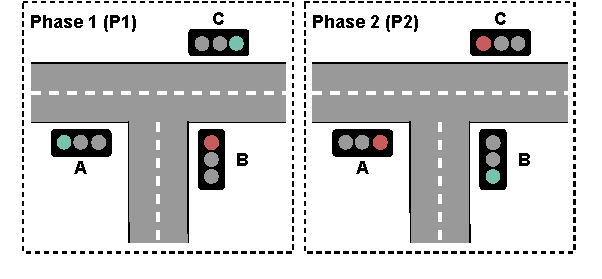
\includegraphics[width=0.5\textwidth]{figures/phases.pdf}
    \caption{Traffic phases of a T-Junction}
    \label{fig:junction-phases}
\end{figure}

To develop the behavior of the traffic management system, we follow an \gls*{mde} approach.
First, we model the behavior of a traffic light as a \gls*{uml} state machine, and then we use \gls*{bpmn} to model the different traffic phases of the T-Junction, including the prioritization of approaching buses.

Using different behavioral modeling languages in the use case has two reasons.
First, two software development teams might work on the system in parallel but prefer different modeling languages.
Second, each team is free to choose the most appropriate modeling language for defining their part of the system.
In this use case, the behavior of a traffic light and a T-Junction differs significantly in complexity and requirements, resulting in the use of two different behavioral modeling languages, namely \gls*{uml} state machines, and \gls*{bpmn}.

The behavior of a traffic light is straightforward since it uses only three colors to guide the traffic.
\autoref{fig:trafficLight} shows the typical European\footnote{Traffic lights in other parts of the world might not show red and amber simultaneously before switching to green.} traffic light that switches from \textsf{red} to \textsf{red-amber}, \textsf{green}, \textsf{amber}, and back to \textsf{red}.
The start state of the traffic light in \cref{fig:trafficLight} is \textsf{red} but can be any of the four possible states.

\begin{figure}[h]
    \centering
    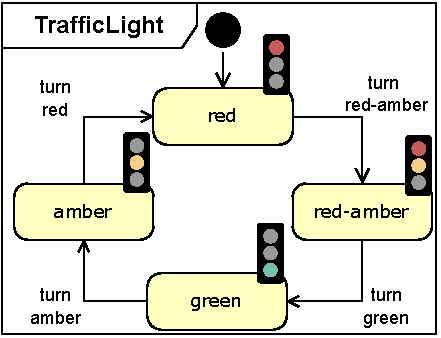
\includegraphics[width=0.35\textwidth]{figures/trafficLight.pdf}
    \caption{Traffic light state machine model}
    \label{fig:trafficLight}
\end{figure}

However, the T-Junction's behavior is more complex since it should coordinate the three traffic lights and communicate with approaching buses to implement bus priority.
Consequently, we are using \gls*{bpmn} to model this aspect of the system's behavior and utilize \gls*{bpmn} message and signal events to implement the communication with approaching buses.

We model two processes, one for the T-Junction and one for the Bus.
Each process is modeled in its own \gls*{bpmn} \emph{pool}.
A pool is depicted as a horizontal lane with a name on the left.
Message flows (arrows with dashed lines) are only allowed between two different pools.

\autoref{fig:t_junction} shows how a possible controller for a T-Junction behaves in the traffic management system.
When a T-Junction controller is started, we assume that the traffic lights are showing the colors according to phase 1 (see \cref{fig:junction-phases}).
Thus, the controller enters a subprocess called phase 1 (see top right in \cref{fig:communication}), which we describe together with the subprocess called phase 2 later.
However, when a fixed amount of time has passed, the subprocess is interrupted by the attached timer boundary event.
Then, the controller executes the next activity and switches to phase 2.
The controller will pass a throwing signal event before entering a subprocess for phase 2 and repeat the same steps.
This signal event represents a broadcast to all buses waiting for traffic light B to become green.
After switching back from phase 2 to phase 1 and signaling that traffic lights A and C are green, the controller can stop or execute the described steps again.
Typically, the controller does not stop, which is indicated by the default sequence flow going back to the process beginning.

% T-Junction BPMN model
\begin{figure*}[h]
    \centering
    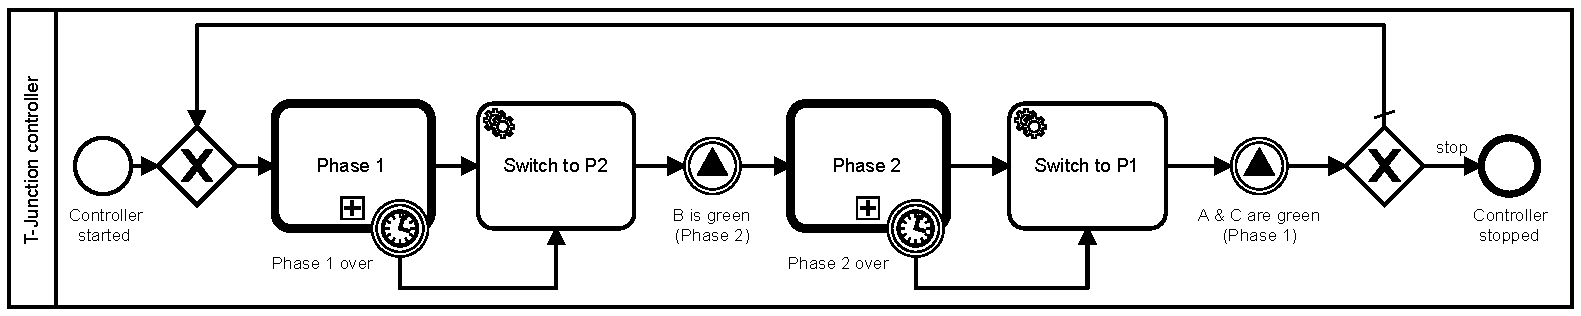
\includegraphics[width=1\textwidth]{figures/t-junction.pdf}
    \caption{Model for a T-Junction controller}
    \label{fig:t_junction}
\end{figure*}

% Bus and Phase 1 BPMN model
\begin{figure*}[ht]
    \centering
    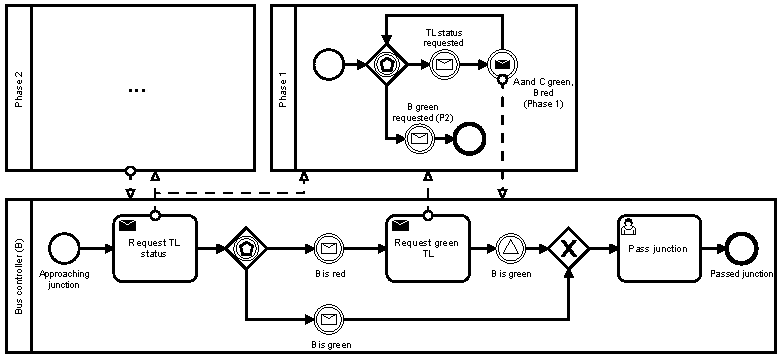
\includegraphics[width=1\textwidth]{figures/communication.pdf}
    \caption{Model for a bus with direction B and its communication with a T-Junction}
    \label{fig:communication}
\end{figure*}

\autoref{fig:communication} shows the communication of a bus with the subprocess phase 1.
The \gls*{bpmn} model and communication for phase 2 of the controller can be defined accordingly.

The phase 1 model uses an event-based gateway to respond to two different kinds of messages.
First, the traffic light status can be requested, which is answered by sending a message declaring that the traffic lights A and C are green while B is red.
Moreover, early green for traffic light B can be requested.
This request ends the subprocess, and the controller immediately switches to phase 2 (see \cref{fig:t_junction}), which results in the traffic light B turning green.

The bottom of \autoref{fig:communication} shows the controller for a bus parameterized with direction B.
It will first request the traffic light status to determine if traffic light B is green.
If it is green, the bus can pass the junction.
However, if it is red, the bus requests to change B to green and waits for a signal that the controller has changed the traffic light.
After receiving the signal, the bus passes the junction.
A \gls*{bpmn} model for a bus controller parameterized with the direction A or C looks nearly identical.
In addition, the bus controller also communicates with the phase 2 subprocess, which we only hint at in \cref{fig:communication}.
The phase 2 subprocess has the same structure as the phase 1 subprocess but reports that A and C are red, while B is green.
Similarly, it terminates if green is requested for A or C.
The full model and all other models are part of the artifacts of this paper \cite{krauterArtifactsBehavioralConsistency2022}.

Having developed behavioral models for the system, we want to check the previously stated \emph{safe traffic} requirement while buses are prioritized.
We can lower the overall development cost if we find bugs related to these requirements as early as possible during system development.
However, the traffic light model is currently not related to the T-Junction and bus models while the T-Junction is supposed to control the traffic lights, for example, when it switches between the two traffic phases.
In addition, the system has to manage multiple slightly different instances of the behavioral models.
For example, there are three traffic lights at one T-Junction starting in different states---i.e., showing different colors---and buses approaching the T-Junction from one of the three directions.
Consequently, we need a model of the system to allow us to define interactions between the models and configure instances of the behavioral models contained in the multi-model.

\begin{figure}[h]
    \centering
    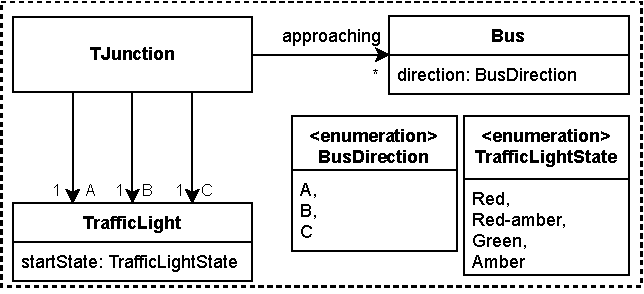
\includegraphics[width=0.45\textwidth]{figures/systemRelationShipModel.pdf}
    \caption{System relationship model of the traffic management system}
    \label{fig:systemRelationshipModel}
\end{figure}

The resulting model called the \textit{\gls*{srm}} is shown in \cref{fig:systemRelationshipModel} using a graph based syntax.
It contains one node for each behavioral model and arrows to depict behavioral relationships, leading to possible interactions.
In addition, it contains enumerations to parameterize the behavioral models. 
A \textsf{TJunction} has three associated \textsf{TrafficLight}s, \textsf{A}, \textsf{B}, and \textsf{C}, and a set of currently approaching \textsf{Bus}es.
A \textsf{TrafficLight} has four possible \textsf{TrafficLightState}s and an attribute to define its \textsf{startState}.
A \textsf{Bus} has a \textsf{direction} that indicates which \textsf{TrafficLight} of the T-Junction it is approaching.

Finally, using the \gls*{srm}, we can define a test configuration of our traffic management system to check its requirements.
\autoref{fig:test_config} depicts the test system configuration as an instance of the \gls*{srm}.
First, it contains three instances of the traffic light behavioral model, representing the three traffic lights, \textsf{A}, \textsf{B}, and \textsf{C}.
Second, it contains an instance of the T-Junction behavioral model, which is connected to the three traffic lights, and two instances of the bus behavioral model.
Thus, the test system configuration describes a system that controls one T-Junction with three traffic lights and two buses approaching from directions A and C.

\begin{figure}[h]
    \centering
    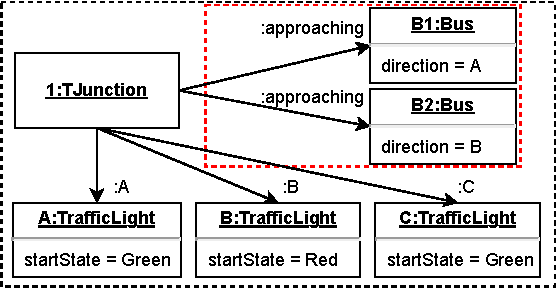
\includegraphics[width=0.45\textwidth]{figures/test_config.pdf}
    \caption{Test system configuration}
    \label{fig:test_config}
\end{figure}

First, we would like to check the safe traffic requirement.
Since we only want to check system conformance concerning the two traffic phases, we do not need to include the two buses depicted in the red dotted square in \cref{fig:test_config} in the analysis.
We cannot simply assert that the system is either in phase 1 or phase 2 since there are intermediate states during the transition between the two phases, which are allowed.
By consulting \cref{fig:trafficLight}, we can, for example, expect a state in which traffic lights A and C are amber, and traffic light B is red-amber before reaching phase 2.
However, we can define \emph{safe traffic} as the absence of \emph{unsafe traffic}, which is easier to define.

For the T-Junction, unsafe traffic occurs if traffic light A is green or amber and traffic light B is green or amber simultaneously.
In addition, the same state combinations are forbidden for traffic lights B and C.
Unsafe traffic occurs only in these situations since green and amber means that cars are allowed to pass, while red (red-amber) means cars are not (not yet, respectively) allowed to pass.
We can formalize the consistency requirements as safety properties in \gls*{ltl}, i.e., states that should never be reached.
The resulting global properties \eqref{eq:property1} and \eqref{eq:property2} are the following, assuming the existence of atomic propositions for each traffic light state. 

\begin{align}
    \square\neg((A_{green} \lor A_{amber}) \land (B_{green} \lor B_{amber})) \label{eq:property1} \\
    \square\neg((C_{green} \lor C_{amber}) \land (B_{green} \lor B_{amber})) \label{eq:property2}
\end{align}

If we include buses \textsf{B1} and \textsf{B2} in the system, we would like to check that they cannot pass when their traffic light is red or red-amber.
Concretely, this means the \textsf{Pass Junction} activity should not execute while the corresponding traffic light is \textsf{red} or \textsf{red-amber}.
We formalize these requirements again by using \gls*{ltl} safety properties \eqref{eq:property3} and \eqref{eq:property4}, where the atomic proposition $B1_{passing}$ and $B2_{passing}$ represent that \textsf{Pass Junction} (see \cref{fig:communication}) has started but not finished yet.

\begin{align}
    \square\neg(B1_{passing} & \land (A_{red} \lor A_{red-amber})) \label{eq:property3} \\
    \square\neg(B2_{passing} & \land (B_{red} \lor B_{red-amber})) \label{eq:property4}
\end{align}

However, to check the global properties, we must execute the system with the behavior specified in the behavioral models according to the test configuration.
This is not straightforward since the multi-model of the use case consists of a \gls*{srm} relating two heterogeneous behavioral models.
In addition, the system configuration instantiates two of the behavioral models multiple times with different parameters.
Furthermore, we face the problem that the models are not independent of each other.
For example, the T-Junction controller must control when the traffic lights A, B, and C switch their states.
Thus, if we were to run the models independently in parallel, the properties would be violated.

% Current approaches can only simulate a set of interacting heterogeneous behavioral models, as discussed in \autoref{sec:introduction}.
% However, they do not allow multiple instances of a behavioral model (without duplicating it) nor provide concrete means to define and check \emph{global} behavioral properties.
% Thus, they are not capable of checking multi-model behavioral consistency.
A multi-model is behaviorally consistent if it satisfies all of its behavioral properties.
A behavioral property is given in temporal logic, for example, \gls*{ltl} in the use case, and is characterized as \emph{local} if it constrains only one model and as \emph{global} if it spans two or more models in a multi-model.
Furthermore, global properties are dependent on the system configuration, i.e., the instance of the \gls*{srm} used.
In the remainder of this paper, we will describe our approach to address behavioral consistency in multi-modeling and apply it to this use case.


\section{Behavioral consistency management} \label{sec:behavioral_consistency_checking}
% Introduce the overall approach using the workflow somehow here and follow it.
\autoref{fig:approach} depicts our approach to behavioral consistency management using a \gls*{bpmn} diagram.

\begin{figure*}[h]
    \centering
    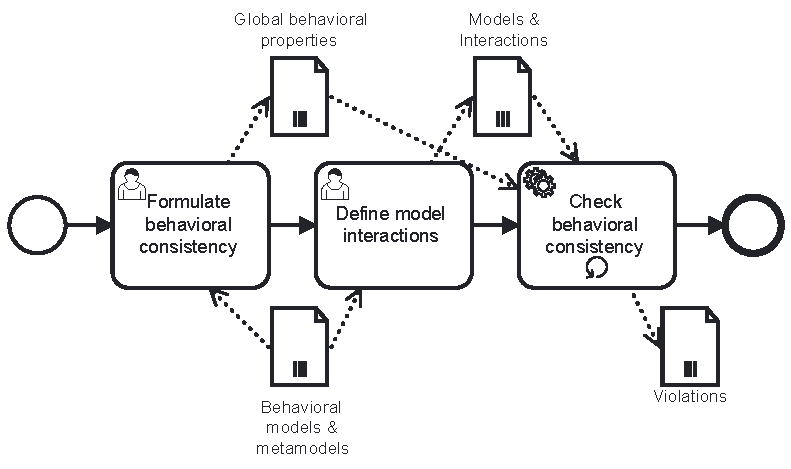
\includegraphics[width=0.7\textwidth]{figures/workflow.pdf}
    \caption{Behavioral consistency management workflow}
    \label{fig:approach}
\end{figure*}

Our approach consists of five steps.
\begin{enumerate}
    \item We define a \glsfirst*{srm} describing which behavioral models may interact.
    \item We specify consistency requirements as global behavioral properties for the \gls*{srm}.
    \item We define interactions between the behavioral models using the \gls*{srm}.
    \item We automatically generate a specification of the specified global behavior using the interactions and the \gls*{srm}.
    \item Given a system configuration we check the global behavioral properties using the generated specification.
\end{enumerate}
The behavioral consistency management workflow potentially uncovers violations, describing counter-examples in which the global behavioral properties are not valid.
In the following sections, we will describe each step in detail.
In addition, the appendix contains \cref{fig:allConcepts}, which gives an overview of all the new concepts and how they are applied to the use case.


\subsection{Define the system relationship model}
As mentioned, a set of behavioral models might be used to describe the behavior of a software system.
Each of these models conforms to its own metamodel which in turn corresponds to the behavioral language used to specify the model.
The metamodel ensures that models specified in the corresponding languages are well-defined and machine-readable.
This is crucial when automating parts of the consistency checking.

The use case utilizes state machine and \gls*{bpmn} models which conform, respectively, to the metamodels of state machines ($M^1$ in \cref{fig:fsm_metamodel}) and \gls*{bpmn} ($M^2$ in \cref{fig:bpmn_metamodel}).
The metamodel of state machines is defined by a \gls*{uml} class diagram with additional information depicted in clouds.
The clouds define a concrete syntax for state machines inspired by \gls*{uml} statecharts.
The traffic light model in \cref{fig:trafficLight} uses this concrete syntax.

% state machine
\begin{figure}[h]
    \centering
    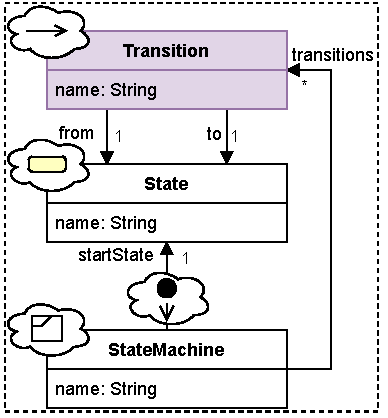
\includegraphics[width=0.275\textwidth]{figures/state_machine_metamodel.pdf}
    \caption{Finite state machine metamodel $M^1$}
    \label{fig:fsm_metamodel}
\end{figure}

A \textsf{StateMachine} has a \textsf{startState} and \textsf{transitions}, whereas each \textsf{Transition} connects two \textsf{State}s.
The states of a state machine are not explicitly modeled but can be derived from the states connected by the transitions of a state machine, assuming no isolated states.

The metamodel for \gls*{bpmn} (see \cref{fig:bpmn_metamodel}) is defined analogous to the one of state machines. 
A \gls*{bpmn} \textsf{Process} contains a set of \textsf{FlowNode}s connected by \textsf{SequenceFlow}s.
\textsf{FlowNode}s and \textsf{SequenceFlow}s are \textsf{FlowElement}s, inheriting an \textsf{id} and a \textsf{name}.
A \textsf{FlowNode} can be an \textsf{Activity}, \textsf{Gateway}, or \textsf{Event}.
Concrete activities, gateways and events are defined in the full \gls*{bpmn} metamodel \cite{objectmanagementgroupBusinessProcessModel2013}. % See BPMN class diagrams in figures 10.104/10.6/10.69.

% BPMN (subset of the needed constructs)
\begin{figure}[h]
    \centering
    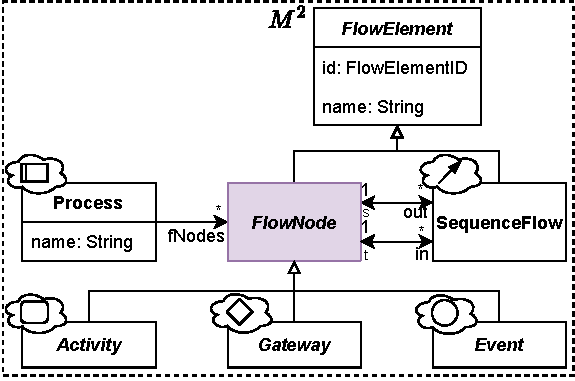
\includegraphics[width=0.475\textwidth]{figures/bpmn_metamodel.pdf}
    \caption{Simplified BPMN metamodel $M^2$ \cite{objectmanagementgroupBusinessProcessModel2013}}
    \label{fig:bpmn_metamodel}
\end{figure}

% System relationship metamodel
Behavioral models \emph{interact} to realize the global system behavior.
A \gls*{srm} describes which behavioral models exist in the system and whether they are behaviorally related; i.e., may interact during execution.
In our approach, we define a system relationship metamodel to formally specify these relationships (see \cref{fig:srm_metamodel_excerpt}).

\begin{figure}[h]
    \centering
    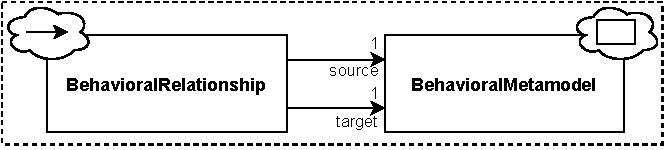
\includegraphics[width=0.45\textwidth]{figures/srm_metamodel_excerpt.pdf}
    \caption{System relationship metamodel excerpt}
    \label{fig:srm_metamodel_excerpt}
\end{figure}
% Also: Behavioral relationships have multiplicities to restrict possible system configurations. But already known for structural models and thus not relevant here.
% Behavioral relationships can be n-ary in the future, not only binary.

We are using a graph based syntax to define \gls*{srm}s (see \cref{fig:systemRelationshipModel}), where each node corresponds to a behavioral model (typed by a \textsf{BehavioralMetamodel}), while each arrow corresponds to a \textsf{BehavioralRelationship} (see concrete syntax depicted in clouds).
For example, the \gls*{srm} for the use case (see \cref{fig:systemRelationshipModel}) has three behavioral relationships from \textsf{TJunction} to \textsf{TrafficLight} since a T-Junction controller interacts with three different traffic lights A, B, and C.
Furthermore, there is a behavioral relationship from \textsf{TJunction} to \textsf{Bus} because we want to check the safety properties \eqref{eq:property3} and \eqref{eq:property4}. 
To summarize, behavioral relationships define \textit{which} behavioral models \textit{may} interact, while the interactions in the next step of the workflow describe \textit{how} they interact.

In addition, we allow enumerations and attributes in \gls*{srm}s.
These may be used as parameters, e.g., to define the start state in a state machine (see \cref{fig:systemRelationshipModel}).
Different instances of the \gls*{srm} can be used to analyze the global behavior of \emph{different} system configurations by changing the parameters.


\subsection{Specify consistency requirements} \label{subsec:specify_consistency_requirements}
In this step, we specify behavioral consistency requirements as global behavioral properties.
These properties are defined using a temporal logic, for example \gls*{ltl} as in the use case.
Temporal logic properties are built upon a set of atomic propositions which are either true or false in a given state.
% To define these global properties, we need a way to represent the states and transitions of the \gls*{srm}
Each behavioral language (e.g. the BPMN) specification defines how these states are represented.
Furthermore, the transitions between these states depend on the semantics of the behavioral models.
In our approach, we call the state representation a \emph{snapshot metamodel} which is specified using class diagrams.

For example, in the use case, we define snapshot metamodels for state machines and \gls*{bpmn}.
A stat machine is in one state at a time, as shown in the snapshot metamodel $M_s^1$ in \cref{fig:fsm_snapshot_metamodel}.
We are reusing the concrete syntax elements from the state machine metamodel $M^1$ in \cref{fig:fsm_metamodel}.
In addition, each snapshot metamodel has a root element in our approach, highlighted in light blue.
\begin{figure}[h]
    \centering
    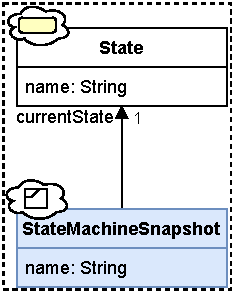
\includegraphics[width=0.25\textwidth]{figures/state_machine_snapshot_metamodel.pdf}
    \caption{Finite state machine snapshot metamodel $M_s^1$}
    \label{fig:fsm_snapshot_metamodel}
\end{figure}

The snapshot metamodel for \gls*{bpmn} is based on a \textsf{Token} distribution as described in the \gls*{bpmn} specifications \cite{objectmanagementgroupBusinessProcessModel2013} (see \cref{fig:bpmn_snapshot_metamodel}). 
% That is, a \emph{snapshot} representing a state of a BPMN model is a distribution of tokens across flow elements. of a process is a set of \textsf{Token}s.
The root element \textsf{ProcessSnapshot} has \textsf{tokens} and \textsf{subprocesses}.
A \textsf{Token} indicates where it is located in the \gls*{bpmn} model using its \textsf{position} attribute.
A valid \textsf{position} is the \textsf{id} of a \textsf{FlowElement} (see \cref{fig:bpmn_metamodel}).
Also for the snapshot metamodel of \gls*{bpmn} we reuse the concrete syntax of the \gls*{bpmn} metamodel.
In addition, \textsf{Token}s are highlighted with green bubbles in the middle of sequence flows and the top right of an activity.

\begin{figure}[h]
    \centering
    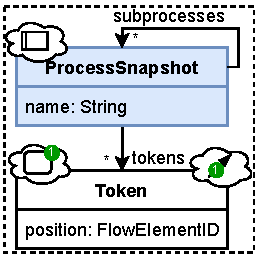
\includegraphics[width=0.25\textwidth]{figures/bpmn_snapshot_metamodel.pdf}
    \caption{BPMN snapshot metamodel $M_s^2$}
    \label{fig:bpmn_snapshot_metamodel}
\end{figure}

% Propositions need the \gls*{srm} and all snapshot metamodels
Using the snapshot metamodels, one can only specify local behavioral properties.
To specify global behavioral properties, we combine the information of the \gls*{srm} with the snapshot metamodels.
Each behavioral model is typed by a behavioral metamodel, which has a snapshot metamodel describing its state structure.
Thus, we know how states of behavioral model are represented, when they are instantiated.
% Use case example propositions
For example, \cref{fig:atomic_propositions} shows how to specify the atomic propositions $A_{green}$ and $B1_{passing}$, used in the global properties in \autoref{sec:usecase}.
Snapshot links connect instances of behavioral models with root element instances of the corresponding snapshot metamodel. 

\begin{figure}[h]
    \centering
    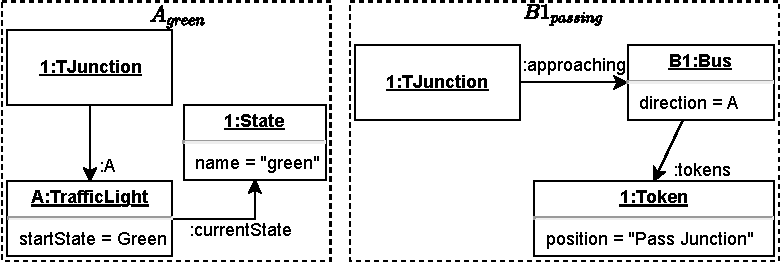
\includegraphics[width=0.475\textwidth]{figures/atomic_props.pdf}
    \caption{Atomic propositions $A_{green}$ and $B1_{passing}$}
    \label{fig:atomic_propositions}
\end{figure}

To make formulating atomic propositions less cumbersome, one can use the concrete syntax of the individual snapshot metamodels.
For example, \cref{fig:atomic_propositions_concrete} shows the same atomic propositions as \cref{fig:atomic_propositions} but uses the introduced concrete syntax.

\begin{figure}[h]
    \centering
    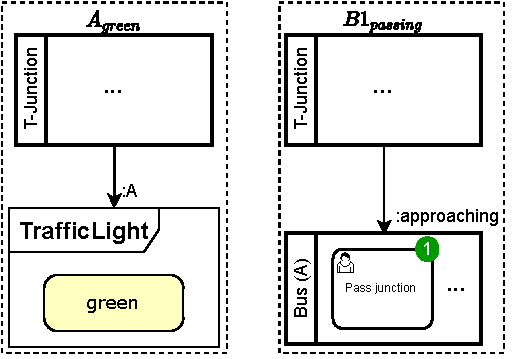
\includegraphics[width=0.4\textwidth]{figures/atomic_props_concrete.pdf}
    \caption{Concrete syntax for $A_{green}$ and $B1_{passing}$}
    \label{fig:atomic_propositions_concrete}
\end{figure}

With the defined atomic propositions as ingredients, one can use temporal logic to define global behavioral properties such as the properties \eqref{eq:property1}-\eqref{eq:property4} in \autoref{sec:usecase}.
It is worth noting that the defined atomic propositions are \textit{model-specific}, meaning they exactly fit the given multi-model.


\subsection{Define model interactions}
Structural models in a multi-model might contain related information.
Thus, current approaches define so-called \emph{commonalities} to explicate these relationships and keep the information consistent \cite{stunkelComprehensiveSystemsFormal2021,klareCommonalitiesPreservingConsistency2019}.

To check the behavioral consistency of a system, we are primarily interested in global system behavior.
However, global behavior depends not only on the local behavior of the models, but also on their interactions.
Consequently, we call these inter-model relationships \emph{interactions} since they carry behavioral meaning while commonalities carry structural meaning \cite{krauterBehavioralConsistencyHeterogeneous2021}.

To specify interactions between different behavioral models, we defined an interaction language given by the full system relationship metamodel in \cref{fig:srm_metamodel}.
In addition, we introduce the concept of \emph{state-changing elements}.
Each \textsf{BehavioralMetamodel} specifies a set of \textsf{StateChangingElement}s.
For example, a state machine defines states and transitions, but only the transitions describe how the states in a state machine change.
Thus, the transitions are the \textsf{StateChangingElement}s of a state machine (highlighted in purple, see \cref{fig:fsm_metamodel}).
Similarly, the flow nodes are the \textsf{StateChangingElement}s of a \gls*{bpmn} process (highlighted in purple, see \cref{fig:bpmn_metamodel})\footnote{One exception is the event-based gateway, which is not part of the \textsf{StateChangingElement}s.}.
The interaction of behavioral models is only possible through instances of the \textsf{StateChangingElement}s.

Our approach is based on the requirement that state-changing elements can be identified in metamodels for any behavioral formalism.
This requirement is not difficult to meet since behavioral modeling languages must have some construct to describe state-change.
Inspecting other behavioral languages, such as Petri Nets or \gls*{uml} activity diagrams, shows that identifying state-changing elements (transitions, activity nodes) is unproblematic. 

\begin{figure}[h]
    \centering
    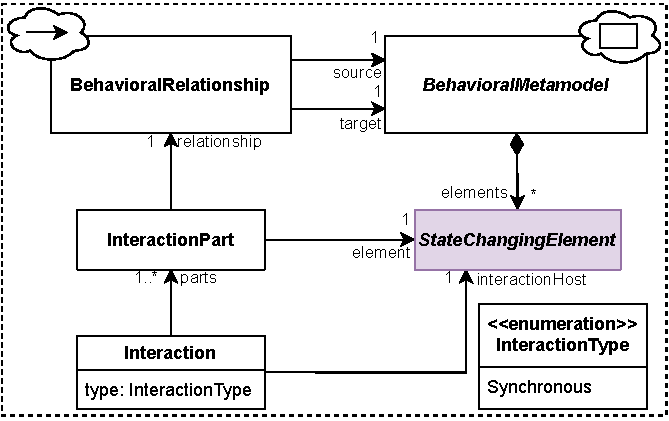
\includegraphics[width=0.475\textwidth]{figures/srm_metamodel_composition.pdf}
    \caption{System relationship metamodel}
    \label{fig:srm_metamodel}
\end{figure}

An \textsf{Interaction} has an \textsf{interactionHost}, a set of interaction \textsf{parts} and an \textsf{InteractionType}.
Currently, there is only the \textsf{synchronous} \textsf{InteractionType}.
However, more interaction types, for example, asynchronous interactions or interactions with message passing, could be added in the future.
Asynchronous interactions can also be modeled using two synchronous interactions with an additional behavioral model, such as a queue.
Each \textsf{InteractionPart} references one \textsf{BehavioralRelationship} and one \textsf{StateChangingElement}.

The \textsf{interactionHost} and the elements of the \textsf{InteractionPart}s describe a state change for their concrete behavioral model.
By connecting them with a synchronous interaction, we define simultaneous state changes in one atomic step. 
Consequently, an interaction can define a synchronization between behavioral models.
In addition, one can only define interactions for state-changing elements if their behavioral models are connected by a behavioral relationship (see constraint \eqref{eq:interactionConstraint}).
We use "." in constraints to navigate along associations.
For example, \textsf{i.parts} means following all \textsf{parts} links for an \textsf{Interaction} object, resulting in a set of \textsf{InteractionPart} objects.

\begin{equation} \label{eq:interactionConstraint}
    \begin{aligned}
    & \forall i \in Interaction: \forall p \in i.parts : \\
    & \quad p.element \in p.relationship.target.elements \; \wedge \\
    & \quad i.interactionHost \in p.relationship.source.elements
    \end{aligned}
\end{equation}

We allow the definition of as many interactions as desired.
The interactions restrict the local behavior of the models since some parts of their behavior must synchronize.
Two interactions are not allowed to share state-changing elements (see constraint \eqref{eq:noOverlap}).
If such a situation occurs, it must be resolved by the modeler by deleting one of the interactions or merging the two interactions into one.

\begin{equation} \label{eq:noOverlap}
    \begin{aligned}
    & \forall i_1,i_2 \in Interaction : \\
    & \quad (i_1.parts.element \cup i_1.interactionHost) \; \cap \\
    & \quad (i_2.parts.element \cup i_2.interactionHost) = \emptyset
    \end{aligned}
\end{equation}

In the use case, the T-Junction controller interacts with the three traffic lights, \textbf{A}, \textbf{B}, and \textbf{C}.
\autoref{lst:interactions} defines two interactions synchronizing T-Junction controller and the traffic lights, using a textual \gls*{dsl}.
The \textbf{synchronize} keyword specifies the \textsf{InteractionType} to be \textsf{synchronous}.

\lstinputlisting[
label=lst:interactions,
language=Interaction,
caption=Interactions for the use case]{figures/interactions.txt}

We can explain the interactions as follows.
The first line defines that the interactions are specified from the viewpoint of the T-Junction in the \gls*{srm} in \cref{fig:systemRelationshipModel}.
The first interaction defines that the task \textsf{Switch to P1} and three other state-changing elements synchronize.
Furthermore, line 3 specifies that one of the synchronization partners is the element \textit{turn green} connected by the relationship \textit{A}.
Similarly, two other transitions of the traffic lights \textit{B} and \textit{C} are specified in the following two lines.
Thus, the interaction defines a synchronization of a task and three traffic light transitions. 
The second interaction defines a synchronization for the task \textsf{Switch to P2} and three traffic light transitions.

To summarize the system relationship metamodel is used to define the relations between the behavioral models in a multi-model.
Thus, the inter-relations between behavioral models in a multi-model are given by interactions and their behavioral relationships.


\subsection{Generate a global behavior specification}
Using the \gls*{srm} and snapshot metamodels, we can represent the global states of the system, but we still need a formal specification of the global behavior to check the defined properties.
The specification of the global behavior used in our approach must fulfill the following three requirements:
\begin{enumerate}
    \item The specification must respect the semantics of each behavioral model, except for interactions.
    \item The specification semantics must reflect the defined interactions between the behavioral models.
    \item The specification semantics must allow the checking of behavioral properties for a given system configuration.
\end{enumerate}
Thus, a specification in any formalism fulfilling these three requirements can be used in our approach.
Consequently, one can experiment with different formalisms, for example, graph transformations, rewriting logic, state machines, Petri nets, or process algebras, without changing the general framework.
One can then pick the most suitable formalism for the modeling scenario at hand regarding, for example, consistency checking performance.
In \cref{sec:specification_of_the_global_behavior}, we describe how we generate specifications for the graph transformation toolset Groove and the Maude system.

To summarize, we generate a specification of the global system behavior.
This generation takes the models and interactions as input and is fully automated to allow frequent model changes.
Regeneration is not needed if only the defined properties change.


\subsection{Check behavioral consistency}
% Model checking for a system configuration
In this step, we use the generated specification of the global behavior to check consistency when given a system configuration.
A system configuration is an instance of the \gls*{srm} and is automatically translated into the formalism of the specification.
We then check the consistency of the defined properties using the specification and the system configuration.
This step is fully automated, such that it can be executed as many times as needed for different system configurations and properties but using the same specification.

Finally, if a consistency requirement is not fulfilled, a violation, including a counterexample, will be presented to the user.
Adopting the same concrete syntax to visualize the counterexample as for the atomic propositions should be ideal for helping a user understand the counterexample. 
An unsuccessful consistency check leads to a consistency restoration process, which is crucial but out of the scope of this paper.
We describe consistency checking for the use case and its result in the end of the next section.


\section{Specification of the global behavior} \label{sec:specification_of_the_global_behavior}
In this section, we will describe our implementation to generate formal specifications in Groove \cite{ghamarianModellingAnalysisUsing2012, rensinkGROOVESimulatorTool2004} and Maude \cite{manuelclavelAllMaudeHighPerformance2007}.
Then, we use the generated specifications to check behavioral consistency for the use case and discuss the results.

Both implementations utilize a \textit{global model transformation} from the behavioral models and their interactions to graph transformation rules (Groove) or rewriting rules (Maude).
We will now describe this transformation generally using the general term \textit{rules} to mean either graph transformation rules or rewriting rules.
The details specific to each implementation are given in the following sections.

The global model transformation can be decomposed into two steps.
The first step to generate a specification of the global behavior is to generate rules for each behavioral model contained in the multi-model.
Each set of rules must describe the behavior of the given behavioral model by manipulating instances of the snapshot metamodels.
For example, a rule for a transition in a state machine changes the current state of a corresponding state machine snapshot from the source to the target state of the transition. 

Thus, we need a \emph{local model transformation} for each behavioral modeling language producing sets of rules.
Each local model transformation only has to be implemented once by an \gls*{mde} tool developer and made available, for example, as a plugin, such that it can then be reused in any future setting the language is needed.
In addition, each local model transformation must keep traces of the generated set of rules.
Concretely, it has to save which rules originated from which state-changing elements in the behavioral model.
Coming back to the state machine example, we must know which transition results in which rule.
In general, multiple rules may be associated with one state-changing element of a behavioral model.
For example, a receive task in a \gls*{bpmn} process is represented by two rules since it starts and then waits for an incoming message before finishing.

The second step is to modify the generated rules to reflect the defined interactions.
Interactions define synchronization of systems which we encode by merging the individual rules into rules describing the global behavior.
The merging process to obtain the global rules is done in two steps:

\begin{enumerate}
    \item Rules generated from state-changing elements that are not part of interactions remain unchanged and are added to the global rule set.
    \item For each interaction, we do the following:
     \begin{enumerate}
         \item Find the corresponding rule\footnote{If one state-changing element results in more than one rule, one can define a strategy to pick the appropriate rule.} $P_0$ for the interaction host of the interaction and find the rules $P_1, P_2, \ldots P_n$ for the state-changing elements taking part in the interaction using the saved traces.
         \item Create a \textit{global rule} for the rules $P_0, P_1, \ldots, P_n$, which applies them simultaneously, i.e., synchronizes the state changes of the behavioral models.
         \item For each part of the interaction, instantiate the corresponding behavioral relationship from the behavioral model in $P_0$ to the behavioral model in $P_i$, for 1 < i $\leq$ n.
         Thus, only behaviorally related models may interact, i.e., change their state simultaneously.
     \end{enumerate}
\end{enumerate}

In the following sections we describe how global rules are created in Groove and Maude.


\subsection{Groove specification} 
% Graph transformation rules and their generation from the behavioral models
This section describes how graph transformations can be used as one possible formalism for behavioral consistency management.
Concretely, we utilize the Groove tool set to run the generated specifications, i.e., graph transformation systems \cite{ghamarianModellingAnalysisUsing2012, rensinkGROOVESimulatorTool2004}.

A graph transformation system consists of a set of graph transformation rules of the form $L \to R$, where the graph $L$ is called left-hand side and the graph $R$ is called right-hand side of the rule.
Nodes/edges in $R$ but not in $L$ are added by a rule, while nodes/edges in $L$ and $R$ are preserved, and a rule deletes nodes/edges that are in $L$ but not in $R$.
Applying a graph transformation system to a given graph one obtains a state space where each state is a graph, and each transition is a rule application.
A formal description of graph transformation systems can, for example, be found in \cite{ehrigFundamentalsAlgebraicGraph2006}. % Section 3.1, especially Definition 3.4.

We generate typed graph transformation systems, where the \gls*{srm} including the snapshot metamodels is the type graph since it fits our rules changing the global state.
Interactions result in global rules which change multiple parts in the global state.
A global rule is given by a parallel production rule \cite[Definition 3.2.7]{baldanConcurrentSemanticsAlgebraic1999} of all individuals rules which essentially results in a pairwise sum of individual rules.
Together with a system configuration, i.e., a start graph, we can obtain an executable formal specification of the global behavior.
Consequently, this can be used to check behavioral consistency.

We will now explain how the graph transformation rules are generated for the use case.
To apply our approach to the use case, we need to define local model transformations from state machines and \gls*{bpmn} processes to graph transformation rules.


\subsubsection{State machine semantics}
The local model transformation to generate graph transformation rules for finite state machines is straightforward.
Each transition leads to a graph transformation rule.
For example, \cref{fig:sm_rules} shows the graph transformation rules for the transitions \textsf{turn red-amber} and \textsf{turn green} of the traffic light model.
It uses the concrete syntax introduced in \cref{fig:fsm_snapshot_metamodel} to depict state machine snapshots and their current states.
We depict a graph transformation rule by showing the graph $L$ on the left, $R$ on the right, and a named white arrow from $L$ to $R$.

\begin{figure}[h]
    \centering
    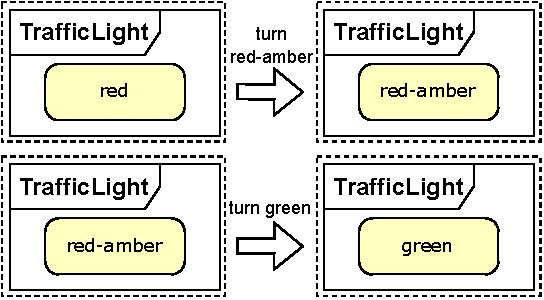
\includegraphics[width=0.3\textwidth]{figures/sm_rules.pdf}
    \caption{Graph transformation rules for \emph{turn red-amber} and \emph{turn green}}
    \label{fig:sm_rules}
\end{figure}

Using a traffic light snapshot with the state red as a start graph, we generate the same state space in Groove as the traffic light state machine describes.
All generated graph transformation systems, including further instructions regarding execution and consistency checking, can be found in \cite{krauterArtifactsBehavioralConsistency2022}.


\subsubsection{BPMN semantics}
The local model transformation to generate graph transformation rules for \gls*{bpmn} processes is challenging, and we are currently only supporting a subset of the \gls*{bpmn} semantics \cite{krauterFormalizationAnalysisBPMN2022}, similar to the extent supported by \cite{vangorpVisualTokenbasedFormalization2013}.
Generally, we construct one or more rules for each flow node in a \gls*{bpmn} model.
\autoref{fig:bpmn_example_rules} shows graph transformation rules for some flow nodes of the T-Junction controller.
It uses the concrete syntax introduced in \cref{fig:bpmn_snapshot_metamodel} to represent process snapshots containing tokens.

\begin{figure}[h]
    \centering
    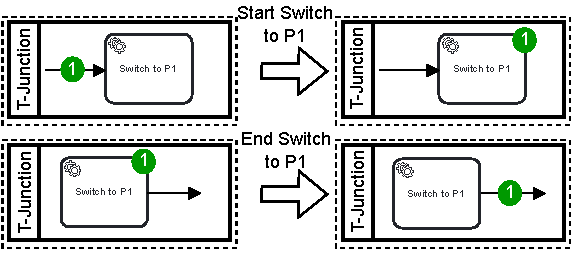
\includegraphics[width=0.475\textwidth]{figures/bpmn_rules.pdf}
    \caption{Example graph transformation rules for the T-Junction controller}
    \label{fig:bpmn_example_rules}
\end{figure}

Due to limited space, we only show a subset of the rules resulting from our \gls*{bpmn} semantics specification.
A detailed explanation of the graph transformation rule generation is given in \cite{krauterFormalizationAnalysisBPMN2022}.

To summarize, we can generate graph transformation systems that implement the behavioral semantics of the \gls*{bpmn}.
Furthermore the artifacts of this paper \cite{krauterArtifactsBehavioralConsistency2022} contain graph transformation systems for the \gls*{bpmn} models of the use case.


% HERE HERE (Adrian stopped reading here)
\subsubsection{Check behavioral consistency}
The defined interactions change the rules for switching to phases 1 and 2.
\autoref{fig:global_rule} shows the resulting rule for switching to phase 1.
We decided that the interactions between the traffic lights and the T-Junction controller should synchronize with the end of the task, not the start.

\begin{figure}[h]
    \centering
    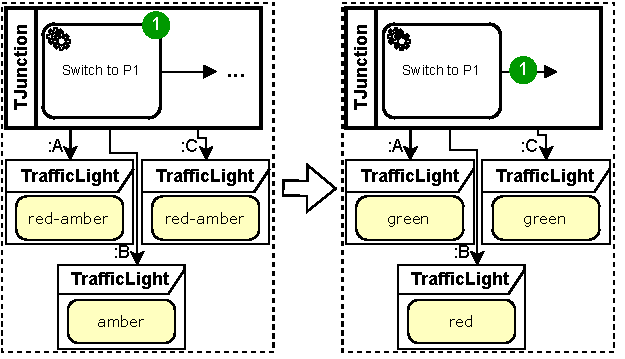
\includegraphics[width=0.475\textwidth]{figures/global_rule.pdf}
    \caption{Global graph transformation rule to switch to phase 1}
    \label{fig:global_rule}
\end{figure}

The rule changes all traffic lights simultaneously and finishes the task.
The corresponding individual rules no longer exist, so synchronization of the behavior is guaranteed.
A similar rule exists for switching to phase 2, resulting from the other interaction.
All other rules are left untouched during the construction of the global graph transformation system.

Finally, we can generate the global state space of the system using the global graph transformation system, which can be found in \cite{krauterArtifactsBehavioralConsistency2022}.
To check the requirements formalized by properties 1-4, we must also encode the used atomic propositions.
These are specified as \textit{graph conditions} in Groove.
A graph condition in Groove is a rule that does not change elements but can be used as an atomic proposition in model checking.


\subsection{Maude specification}
We are using the predefined Maude module for object-based programming to encode the snapshot metamodels in Maude.
Thus, we can represent state machine snapshots and \gls*{bpmn} process snapshots as objects in Maude.
In addition, we add behavioral relationships from the \gls*{srm} such that we can instantiate them to create the system configuration described in the use case.

Our Maude rules always rewrite multisets of objects, where individual objects are denoted in angle brackets ($<\cdots>$).
Interactions lead to rule merges in Maude, where the left and right side of each rule is added to a global rule.
The global rule is a valid Maude rule since the union of two multisets always results in a multiset. 
Furthermore, behavioral relationships as defined in the interaction, are added to the rule as additional objects on both sides.
Similarly to the process for graph transformation rules, individual rules are deleted.

We will now explain how rewriting rules are generated for the use case.
To apply our approach to the use case, we need to define local model transformations from state machines and \gls*{bpmn} processes to rewriting rules.


\subsubsection{State machine semantics}
The generation of rewriting rules is similar to the generation of graph transformation rules.
Each state machine transition leads to one rewriting rule, which rewrites state machines conforming to the state machine snapshot metamodel.
\autoref{lst:trafficLightMaude} shows the rewriting rules for the traffic light model.
For example, line 3-4 defines a rewriting rule \textsf{turn\_red\_amber}, which changes the state of a traffic light object from red to red-amber.

In addition to the rewriting rules, a start configuration is generated based on the defined start state (see lines 7 and 8).
The start configuration is the Maude counterpart of the start graph in graph transformation systems.

\lstinputlisting[
label=lst:trafficLightMaude,
language=Interaction,
float=*,
caption=Rewriting rules and start configuration for a traffic light]{figures/trafficLight.maude}

Using Maude's search command and search graph visualization, we can verify that the generated state space conforms to the traffic light state machine.
The generated Maude specifications and example Maude executions can be found in \cite{krauterArtifactsBehavioralConsistency2022}.

\subsubsection{BPMN semantics}
The rewriting rule generation is similar to the graph transformation rule generation and supports the same subset of \gls*{bpmn} semantics.
Similarly, one or more rules are constructed for each flow node in a \gls*{bpmn} process, where objects conform to the \gls*{bpmn} snapshot metamodel.
\autoref{lst:tJunctionControllerMaude} shows two Maude rewriting rules for the first two flow nodes of the T-Junction controller as depicted in \cref{fig:bpmn_example_rules}.
The remaining rules can be found in \cite{krauterArtifactsBehavioralConsistency2022}.
For example, the rule \textsf{Controller\_started} from line 5 to line 11 moves a token from the controller started start event to the outgoing sequence flow by changing the token position.
All other attributes of the \textsf{ProcessSnapshot} remain unchanged by the rule.

\lstinputlisting[
label=lst:tJunctionControllerMaude,
language=Interaction,
float=*,
caption=Example rewriting rules for the T-Junction controller]{figures/tJunctionController.maude}

\lstinputlisting[
label=lst:synchRuleMaude,
language=Interaction,
float=*,
caption=Global Maude rule to switch to phase 1]{figures/synch.maude}

Like the graph transformation rules, the rewriting rules move tokens by changing their position according to the given \gls*{bpmn} model.
Thus, we can generate Maude rewriting rules that implement the behavioral semantics of the \gls*{bpmn} models in the use case (see \cite{krauterArtifactsBehavioralConsistency2022}).

\subsubsection{Check behavioral consistency}
The defined interactions change the rules for switching to phases 1 and 2. \autoref{lst:synchRuleMaude} shows the resulting rule for switching to phase 1, where a synchronization with the end of the task was chosen.
\autoref{fig:global_rule} shows the equivalent graph transformation rule.

% lst:synchRuleMaude should be here but moved highter due to formatting

The rule changes all traffic lights simultaneously and finishes the task.
Similarly, a global rule for switching to phase 2 is created and all individual rules are deleted.

Finally, we can use the Maude model checker module to check the requirements formalized by the \gls*{ltl} properties 1-4.
Atomic propositions can be represented in Maude using the encoded \gls*{srm} and the snapshot metamodels.


\subsection{Behavioral consistency in the use case}
Both specifications show that properties 1 and 2 hold, while properties 3 and 4 do \textit{not} hold (see artifacts in \cite{krauterArtifactsBehavioralConsistency2022}).
The counterexamples for properties 3 and 4 show an unexpected race condition that must be handled.
After the T-Junction controller signals that the traffic light A/B is green, bus B1/B2 can advance to the \textsf{Pass Junction} activity.
However, at the same time, the T-Junction controller can enter the subprocess for the next phase, which can be interrupted by the associated timer event.
This can happen before the bus B1/B2 passes the junction, resulting in an invalid state.

The system developers have different options to handle the uncovered inconsistencies.
One option is to keep the models unchanged and pay special attention to the found race condition during system implementation.
This can be an acceptable solution since the \textsf{Pass Junction} activity is also modeled as a user activity, i.e., the bus driver decides when to cross the T-Junction.
Furthermore, tolerating inconsistencies can be a viable option in \gls*{mde} \cite{weidmannToleranceModelDrivenEngineering2021}.
Another option is to change the models to resolve the inconsistency.
For example, the T-Junction controller could wait for the bus to pass before changing the traffic lights again.


\section{Related work} \label{sec:related_work}
This contribution builds on our previous publication \cite{krauterBehavioralConsistencyHeterogeneous2021}.
However, we refined the behavioral consistency management workflow by introducing new concepts such as the \gls*{srm} and snapshot metamodel.
Moreover, we created an interaction language and outlined a general approach to define atomic propositions, leading to global behavioral properties.
In addition, our previous work did not support \gls*{bpmn} models.

% Highlight some specific combinations/ad-hoc approaches for a single modeling language.
The general idea of transforming different behavioral formalisms to a single semantics domain to reason about cross-cutting concerns is not new, see, e.g. \cite{engelsMethodologySpecifyingAnalyzing2001}.
For example, \cite{kusterExplicitBehavioralConsistency2003} developed consistency checking for sequence diagrams and statecharts based on \gls*{csp}, while \cite{yaoConsistencyCheckingUML2006} used Petri nets for the same scenario.
Furthermore, \cite{cunhaFormalVerificationUML2011} analyze sequence diagrams in the context of embedded systems using a transformation to Petri nets.
Nevertheless, all approaches focus on a single modeling language or a fixed combination of two languages.
Consequently, they do not consider the general problem of behavioral consistency in a heterogeneous modeling scenario.

% Kienzle with event structures
\cite{kienzleUnifyingFrameworkHomogeneous2019} proposes a unifying framework for homogeneous model composition.
To combine behavioral models, they use Event structures \cite{winskelEventStructures1987} as an underlying formalism and show how different homogeneous behavioral models can be combined.
Nonetheless, they do not apply their approach to heterogeneous models.
Generally, their approach is compatible with ours since we do not mandate a specific formalism in our approach.
However, we have chosen graph transformation rules as the first formalism to use in our approach since they operate on a higher abstraction level.
In addition, it was shown that many formalisms, for example, the $\pi$-calculus \cite{gadducciGraphRewritingPcalculus2007}, can be implemented using graph transformation rules.

% Gemoc Studio/BCOOL?
\cite{deantoniModelingBehavioralSemantics2016} tackles the problem of dealing with relationships between heterogeneous behavioral models.
They coordinate the different models using their coordination language B-COoL \cite{varalarsenBehavioralCoordinationOperator2015}, similar to the interactions we define between behavioral models.
To execute the models and their coordination, they transform them into \gls*{ccsl} models.  
Their work also results in plugins for GEMOC studio, which support running and debugging the models.
% Ptolemy
\cite{ekerTamingHeterogeneityPtolemy2003, leeDisciplinedHeterogeneousModeling2010} propose an actor-oriented solution to the model composition problem in the presence of heterogeneity.
Their approach results in the tool Ptolemy \cite{ptolemaeusSystemDesignModeling2014}.

% very nice, but only simulation for Ptolemy and no real verification support (LTL model checking and atomic prop definition) in BCool/Gemoc.
However, both approaches focus on simulation rather than consistency or model-checking.
Neither provides concrete means to define atomic propositions and check global behavioral properties.


\section{State space explosion} \label{sec:state_space_explosion}
State space explosion is one of the predominant issues when applying model checking to complex systems, as they are often found in real-world applications.
As one can see in \cref{table:grooveRuntime} and \cref{table:maudeRuntime} our approach is not immune to state space explosion.
The tables show the states, transitions (rewrites), and average runtime of a full state space exploration in the Groove (Maude) specification.
Four scenarios were benchmarked, starting with the use case multi-model without approaching buses and then increasing the number of buses up to three.

To calculate the average runtime, we used the hyperfine benchmarking tool \cite{peterHyperfine2022} (version 1.15.0), which ran state space exploration for each scenario ten times.
Timing evaluations were done on a notebook with an AMD Ryzen PRO 3500U processor and 16 GB of RAM running Maude version 3.2.1 (inside the Windows Subsystem for Linux) and Groove version 5.8.1.
A description how to run the benchmarks is available in \cite{krauterArtifactsBehavioralConsistency2022}.

The benchmarks include start-up times, for example, the state space exploration for the \textsf{No Buses} scenario takes \textasciitilde 500ms according to Groove.
Thus, most of the exploration time in Groove and Maude for the \textsf{No Buses} scenario is attributed to the start-up time.
Generally, the Maude exploration time is lower despite larger state spaces due to technical differences in implementing the \gls*{bpmn} semantics.
However, as expected, neither of the tools is immune to state space explosion.

\begin{table}
\centering

\begin{tabular}{|c || c | c | c |}
 \hline
 Use case & States & Transitions & Exploration time \\
 \hline\hline
 No buses & 168 & 438 & \textasciitilde 2.948 ms \\
 \hline
 1 bus & 2.888 & 10.046 & \textasciitilde 4.510 ms \\
 \hline
 2 buses & 27.880 & 121.554 & \textasciitilde 11.629 ms \\
 \hline
 3 buses & 195.336 & 1.028.340 & \textasciitilde 63.487 ms \\
 \hline
\end{tabular}
\caption[State space exploration in Groove]{State space exploration in Groove}
\label{table:grooveRuntime}

\bigskip

\begin{tabular}{|c || c | c | c |}
 \hline
 Use case & States & Rewrites & Exploration time \\
 \hline\hline
 No buses & 168 & 664 & \textasciitilde 63.3 ms \\
 \hline
 1 bus & 3.304 & 19.958 & \textasciitilde 277.8 ms \\
 \hline
 2 buses & 35.280 & 27.9776 & \textasciitilde 2.994 ms \\
 \hline
 3 buses & 260.176 & 2.522.582 & \textasciitilde 28.091 ms \\
 \hline
\end{tabular}
\caption[State space exploration in Maude]{State space exploration in Maude}
\label{table:maudeRuntime}

\end{table}

% Discussion
% Full state space is not what you do. You check properties.
As in our use case, one is generally not interested in a full state space exploration as in \cref{table:grooveRuntime} and \cref{table:maudeRuntime} but rather in the validity of a set of behavioral properties.
Checking, for example, a property specified in \gls*{ltl}, does not necessarily lead to a full state space exploration.
Furthermore, not every property is concerned with all behavioral models.
For example, properties (1) and (2) of the use case do not involve buses and can be checked on the much smaller state spaces, not including approaching buses.
In addition, checking a set of properties can be run in parallel.
If some properties show to be computationally expensive, they can be run on dedicated hardware, for example, during a continuous integration pipeline once a day in case of behavioral model or interaction changes.
Thus, checking the consistency of a multi-model can be seen as an additional test during \gls*{mde}, which can be run locally but, in addition, is a vital part of continuous integration.

% Ways to mitigate state space explosion.
The Maude \gls*{ltl} model-checker has performance comparable to the popular SPIN model checker \cite{ekerMaudeLTLModel2004} and thus is proven to have a good performance.
However, one could use different techniques to mitigate the state space explosion problem further.
One technique is to abstract models further such that they only contain information relevant to the set of properties to be checked.
Thus, minimal models are synchronized, leading to smaller state spaces.
However, finding correct minimal models might not be trivial.

Partial-order reduction is a well-known and successful technique to mitigate the state space explosion problem.
It is currently not implemented in the Maude LTL model-checker, but there is promising work to integrate partial-order reduction into the model-checker \cite{farzanPartialOrderReduction2007}, showing substantial state space reductions.
The potential to reduce the state space using this technique is huge, especially for model-checking concurrent systems \cite{clarkeHandbookModelChecking2018}.
Our approach analyzes concurrent systems with some interaction, and thus model-checking would greatly benefit from partial-order reduction.
In our opinion, partial-order reduction must be implemented to analyze models from real-world applications.


\section{Conclusion and future work} \label{sec:conclusion_and_future_work}
% Conclusion
Our work represents the first general fully-formalized approach to behavioral consistency management in a heterogeneous modeling scenario, enabling formulating and checking \emph{global} properties.
Previous work either only dealt with the behavioral consistency between specific pairs of models \cite{yaoConsistencyCheckingUML2006, kusterExplicitBehavioralConsistency2003} or focused on the simulation in a heterogeneous scenario \cite{deantoniModelingBehavioralSemantics2016, varalarsenBehavioralCoordinationOperator2015, ekerTamingHeterogeneityPtolemy2003, leeDisciplinedHeterogeneousModeling2010}.

Our approach follows three key steps (see \cref{fig:approach}).
% Describe the three steps
First, we specify global behavioral consistency requirements based on the given behavioral models and their relationships. 
Then, we align the behavioral models by defining their interactions.
Finally, we can check the global consistency of the system in different configurations with the given consistency requirements by generating a formal specification of the global behavior.
The global behavior specification is based on the defined interactions but preserve the original behavior of each model besides interactions.
In addition, not only fully automatized model-checking but also a user-driven simulation of the multi-model and its interactions is possible.
Our approach is independent of the particular formalism used in the generated specification, and we currently support generating graph transformations (Groove) and rewriting logic (Maude).
The successful implementation shows that our approach can work with different underlying formalisms and serves as a \textit{proof of concept}.
Furthermore, we discussed the state space explosion problem and how it can be mitigated.

In future work, extending our implementation to include other behavioral formalisms such as activity diagrams, hierarchical state machines, and the $\pi$-calculus is interesting.
Especially integrating the $\pi$-calculus, which was formalized using graph transformation systems in \cite{gadducciGraphRewritingPcalculus2007}, will be beneficial since it is profoundly different from the currently supported formalisms.

% Data transfer
Furthermore, two systems often exchange data while interacting, for example, using messaging.
The exchanged data then greatly influences the future behavior of the systems.
Thus, adding data transfers to interactions between heterogeneous models is an important issue left for future work.

% Multi-model runtime verification
In addition, it is important to check that running systems are behaving as specified in their behavioral models, including the defined interactions between them.
Thus, extending runtime verification techniques to include systems specified by a multi-model with interactions constitutes a challenging problem.

% Consistency restoration
%We leave potential consistency restoration as a problem for future work.
Finally, once  uncovers consistency violations, consistency restoration must be achieved.
Results from the consistency checking step play a fundamental role for semi-automatic consistency restoration. % Cite something

\bibliography{bib}


\section*{About the authors}

\shortbio{Tim Kräuter}{is a Ph.D. student at the Western Norway University of Applied Sciences, Bergen, Norway.
His primary research is on integrating heterogeneous behavioral models in multi-model-driven software engineering.
Previously he worked as a software developer at SET GmbH in Germany and acquired a master of science in Information Engineering at the University of Applied Sciences, FHDW Hannover, Germany.
\authorcontact[https://timkraeuter.com/]{tkra@hvl.no}}

\shortbio{Harald König}{is a professor for Computer Science at the University of Applied Sciences, FHDW Hannover, Germany, and an Adjunct Professor at the Department of Computer Science, Electrical Engineering and Mathematical Sciences at the Western Norway University of Applied Sciences, Bergen, Norway.
Before entering academia, he worked at SAP in Walldorf and received his Ph.D. in pure Mathematics from Leibniz University in Hannover, Germany. \authorcontact{harald.koenig@fhdw.de}}

\shortbio{Adrian Rutle}{is a professor at the Department of Computer science, Electrical engineering and Mathematical sciences at the Western Norway University of Applied Sciences, Bergen, Norway.
Rutle’s main interest is applying theoretical results from the field of model-driven software engineering to practical domains and has his main expertise in the development of formal modeling frameworks for domain-specific modeling languages, graph-based logic for reasoning about static and dynamic properties of models, and the use of model transformations for the definition of the semantics of modeling languages.
His recent research focuses on multilevel modeling, model repair, multi-model consistency management, modeling and simulation for robotics, digital fabrication, smart systems, and applications of machine learning in model-driven software engineering.
\authorcontact{aru@hvl.no}}

\shortbio{Yngve Lamo}{is a professor at the Department of Computer science, Electrical engineering and Mathematical sciences at the Western Norway University of Applied Sciences, Bergen.
Lamo holds a Ph.D. in Computer Science from the University of Bergen, Norway. His research interests span from formal foundations of Model Based Software Engineering to its applications, especially in Health Informatics.
He is currently applying MDSE to create Adaptive Software Technologies for mental Health. \authorcontact{yla@hvl.no}}

\shortbio{Patrick Stünkel}{is currently working as a postdoctoral researcher at Haukeland University Hospital in Bergen, Norway, where he is working on applying process mining, workflow modeling, and optimization techniques in digital pathology.
Before that, Patrick did his Ph.D. at Western Norway University of Applied Sciences on the topics of semantic interoperability and consistency management among heterogeneous software models.
\authorcontact[https://past.corrlang.io/]{Patrick.Stunkel@helse-bergen.no}}

% \section*{Appendix}

\begin{figure*}[ht]
    \centering
    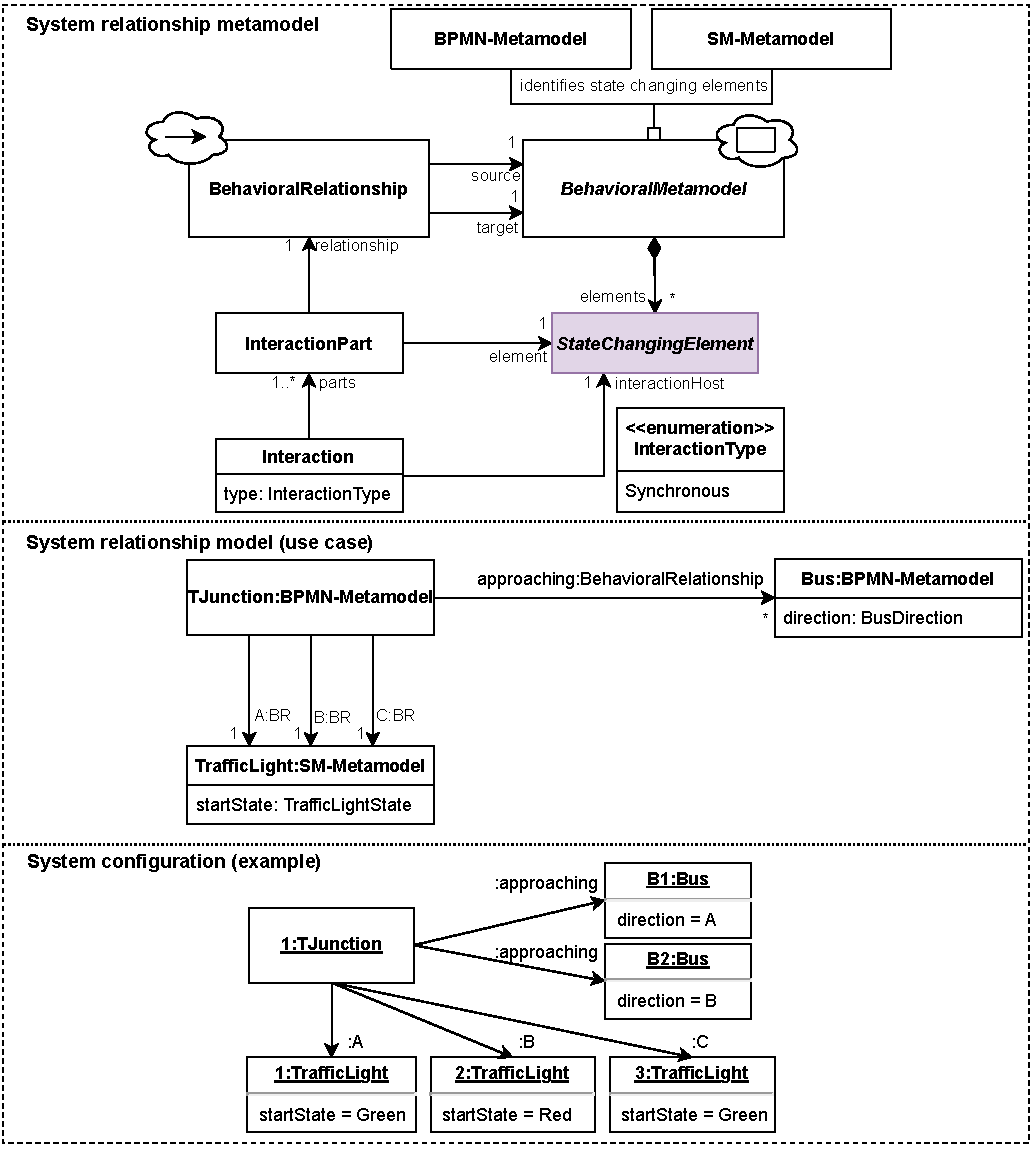
\includegraphics[width=1\textwidth]{figures/allConcepts_composition.pdf}
    \caption{Overview of all concepts and their usage in the use case}
    \label{fig:allConcepts}
\end{figure*}

\end{document}